\documentclass[11pt,a4paper]{article}

% ---------- Packages ----------
\usepackage[margin=1in]{geometry}
\usepackage{amsmath,amssymb,amsthm,mathtools}
\usepackage{booktabs}
\usepackage{array}
\usepackage{xcolor}
\usepackage{enumitem}
\usepackage{titlesec}
\usepackage{caption}
\usepackage{tikz}
\usetikzlibrary{arrows.meta,positioning}
\usepackage[hidelinks]{hyperref}

% ---------- Theorem-like environments ----------
\newtheorem{definition}{Definition}[section]
\newtheorem{example}{Example}[section]

% ---------- Section styling ----------
\titleformat{\section}{\normalfont\Large\bfseries}{\thesection}{1em}{}
\titleformat{\subsection}{\normalfont\large\bfseries}{\thesubsection}{1em}{}

\newcommand{\ind}{\perp\!\!\!\perp}

\title{\textbf{Bayesian and Frequentist Approaches to Statistical Inference:\\ A Detailed Comparative Review}}
\author{}
\date{\today}

\begin{document}

\maketitle

\begin{abstract}
\noindent Statistical inference rests on two dominant, historically competing paradigms: the frequentist approach, which defines probability as long-run frequency and treats unknown parameters as fixed constants, and the Bayesian approach, which defines probability as a coherent measure of belief and treats unknown parameters as random variables governed by a probability distribution. This review develops both frameworks from their philosophical foundations through point and interval estimation, hypothesis testing, model selection, and computation. A worked example (estimating a binomial proportion) is carried through the entire document to make the comparison concrete. The review closes with a discussion of asymptotic equivalence, hybrid methodologies, and practical guidance for choosing between the two paradigms.
\end{abstract}

\tableofcontents

% ============================================================
\section{Introduction}
% ============================================================
Every statistical procedure -- a confidence interval, a $p$-value, a regression coefficient -- is built on top of an answer to a deceptively simple question: \emph{what does probability mean?} The frequentist and Bayesian schools answer this question differently, and the disagreement cascades through every subsequent step of inference: how parameters are conceived, how uncertainty is quantified, how evidence is weighed, and how conclusions are communicated.

This is not merely an academic dispute. The two paradigms can lead to different point estimates, different interval estimates, and even different conclusions from identical data, particularly in small samples or under sequential (optional-stopping) designs. Understanding both frameworks -- their assumptions, their guarantees, and their failure modes -- is essential for using either one responsibly.

The remainder of this review is organized as follows. Section~2 lays out the philosophical foundations and brief history of each school. Section~3 gives the formal mathematical setup. Sections~4--6 compare point estimation, interval estimation, and hypothesis testing. Section~7 discusses the role of the prior distribution in Bayesian inference. Section~8 compares model selection criteria. Section~9 discusses computation. Section~10 works a single example (a binomial proportion) through both frameworks side by side. Section~11 summarizes strengths and weaknesses. Section~12 discusses asymptotic reconciliation between the two schools, and Section~13 concludes.

% ============================================================
\section{Philosophical Foundations}
% ============================================================

\subsection{The Frequentist Interpretation of Probability}
Under the frequentist interpretation, the probability of an event is the limiting relative frequency with which it would occur in an indefinitely repeated sequence of identical trials:
\begin{equation}
P(A) = \lim_{n \to \infty} \frac{\#\{\text{times } A \text{ occurs in } n \text{ trials}\}}{n}.
\end{equation}
Probability is therefore only meaningfully attached to events that are (at least in principle) repeatable. A fixed, unknown population parameter $\theta$ -- the true mean height of a species, the true effect of a drug -- is \emph{not} a random quantity under this view: it has one true value, and it is the data, not the parameter, that is random. Statements of uncertainty are consequently statements about the behavior of a procedure over hypothetical repetitions of the experiment, not about $\theta$ itself.

\subsection{The Bayesian Interpretation of Probability}
Under the Bayesian interpretation, probability is a coherent, numerical measure of a rational agent's degree of belief in a proposition, whether or not that proposition concerns a repeatable event. Because a fixed but unknown parameter $\theta$ can be believed-in to varying degrees, it is legitimate -- indeed central -- to assign $\theta$ a probability distribution. This distribution does not claim that $\theta$ is physically random; it encodes the observer's uncertainty about its value. Observing data updates this belief distribution via Bayes' theorem, producing a posterior distribution that combines prior knowledge with the evidence in the data.

\subsection{Historical Development}
Inverse probability -- reasoning from observed effects back to their causes -- dates to Bayes's posthumously published essay (1763) and was substantially developed by Laplace, who used what would now be called Bayesian methods with uniform priors as a matter of course. In the early twentieth century, R.A.~Fisher, and later Jerzy Neyman and Egon Pearson, objected to the reliance on subjective priors and built an alternative foundation using only the sampling distribution of the data: maximum likelihood estimation, significance testing, and the Neyman--Pearson theory of hypothesis testing. This frequentist program came to dominate applied statistics for most of the twentieth century, aided by the fact that its calculations were tractable by hand or with early computers, whereas Bayesian posteriors for anything but simple conjugate models generally were not.

Harold Jeffreys kept the Bayesian tradition alive through the mid-twentieth century, developing objective priors invariant under reparameterization. The Bayesian approach was reinvigorated from the 1990s onward by the development and popularization of Markov chain Monte Carlo (MCMC) methods, which made it computationally feasible to approximate posterior distributions for complex, high-dimensional models. Today both paradigms are in wide active use, and much of applied statistics and machine learning draws on ideas from both.

% ============================================================
\section{Formal Frameworks}
% ============================================================

\subsection{The Frequentist Framework}
Let $X_1, \dots, X_n$ be a random sample from a distribution with density (or mass function) $f(x; \theta)$, where $\theta \in \Theta$ is a fixed, unknown constant. All frequentist inference is based on the \emph{sampling distribution} of statistics computed from the data -- that is, on the distribution the statistic would have if the experiment were repeated indefinitely under the same conditions with $\theta$ held fixed. An estimator $\hat\theta = \hat\theta(X_1,\dots,X_n)$ is itself a random variable, since it is a function of the (random) data; $\theta$ is never random.

\subsection{The Bayesian Framework}
The Bayesian framework treats $\theta$ as a random variable and requires three ingredients:
\begin{itemize}[leftmargin=2em]
  \item a \textbf{prior distribution} $\pi(\theta)$, encoding beliefs about $\theta$ before observing data;
  \item a \textbf{likelihood} $L(\theta ; x) = f(x ; \theta)$, the same sampling model used by frequentists, now read as a function of $\theta$ for fixed data $x$;
  \item Bayes' theorem, which combines the two into a \textbf{posterior distribution}:
\end{itemize}
\begin{equation}
\pi(\theta \mid x) \;=\; \frac{L(\theta; x)\, \pi(\theta)}{m(x)}, \qquad m(x) = \int_{\Theta} L(\theta; x)\, \pi(\theta)\, d\theta,
\label{eq:bayes}
\end{equation}
where $m(x)$ -- the \emph{marginal likelihood} or \emph{evidence} -- normalizes the posterior so that it integrates to one. Equation~\eqref{eq:bayes} is often abbreviated
\begin{equation}
\pi(\theta \mid x) \;\propto\; L(\theta;x)\,\pi(\theta), \qquad \text{i.e.\ posterior} \propto \text{likelihood} \times \text{prior}.
\end{equation}

\begin{center}
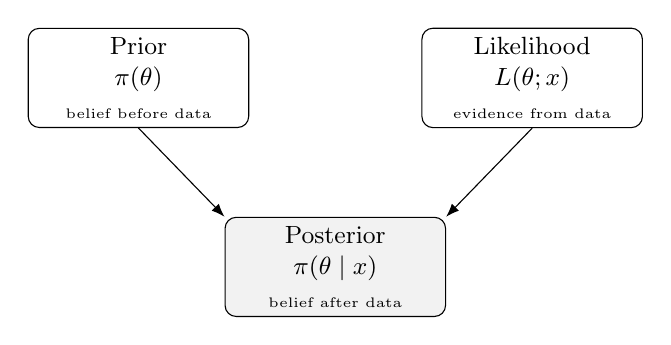
\begin{tikzpicture}[>=Latex, box/.style={draw, rounded corners, minimum width=2.8cm, minimum height=1cm, align=center, font=\small}]
  \node[box] (prior) at (0,2.4) {Prior\\ $\pi(\theta)$\\[1pt] \tiny belief before data};
  \node[box] (lik) at (5,2.4) {Likelihood\\ $L(\theta;x)$\\[1pt] \tiny evidence from data};
  \node[box, fill=gray!10] (post) at (2.5,0) {Posterior\\ $\pi(\theta\mid x)$\\[1pt] \tiny belief after data};
  \draw[->] (prior.south) -- (post.north west);
  \draw[->] (lik.south) -- (post.north east);
\end{tikzpicture}
\end{center}

\begin{definition}[Conjugate prior]
A prior $\pi(\theta)$ is \emph{conjugate} to a likelihood $L(\theta;x)$ if the resulting posterior $\pi(\theta\mid x)$ belongs to the same parametric family as the prior. Conjugate priors allow the posterior to be written in closed form and are used extensively in Section~10.
\end{definition}

% ============================================================
\section{Point Estimation}
% ============================================================

\subsection{Frequentist Point Estimation}
The dominant frequentist point estimator is the \textbf{maximum likelihood estimator (MLE)},
\begin{equation}
\hat\theta_{\text{MLE}} = \operatorname*{arg\,max}_{\theta \in \Theta} L(\theta; x).
\end{equation}
Estimators are judged by properties of their sampling distribution:
\begin{itemize}[leftmargin=2em]
  \item \textbf{Bias}: $\operatorname{Bias}(\hat\theta) = E_\theta[\hat\theta] - \theta$; an estimator is unbiased if this is zero for all $\theta$.
  \item \textbf{Variance} and \textbf{Mean Squared Error}: $\operatorname{MSE}(\hat\theta) = \operatorname{Var}(\hat\theta) + \operatorname{Bias}(\hat\theta)^2$.
  \item \textbf{Consistency}: $\hat\theta_n \xrightarrow{P} \theta$ as $n \to \infty$.
  \item \textbf{Efficiency}: an unbiased estimator is efficient if its variance attains the Cram\'er--Rao lower bound, $\operatorname{Var}(\hat\theta) \ge 1/I_n(\theta)$, where $I_n(\theta)$ is the Fisher information.
  \item \textbf{Asymptotic normality}: under regularity conditions, $\sqrt{n}(\hat\theta_{\text{MLE}} - \theta) \xrightarrow{d} N\!\big(0,\, I(\theta)^{-1}\big)$.
\end{itemize}

\subsection{Bayesian Point Estimation}
A Bayesian point estimate is obtained by minimizing the \emph{posterior expected loss} for a chosen loss function $L(\theta, a)$:
\begin{equation}
\hat\theta_{\text{Bayes}} = \operatorname*{arg\,min}_{a} \; E\big[L(\theta, a) \mid x\big] = \operatorname*{arg\,min}_{a} \int_\Theta L(\theta, a)\, \pi(\theta \mid x)\, d\theta.
\end{equation}
The choice of loss determines the summary of the posterior that is reported:
\begin{itemize}[leftmargin=2em]
  \item squared error loss $\Rightarrow$ the \textbf{posterior mean} $E[\theta \mid x]$;
  \item absolute error loss $\Rightarrow$ the \textbf{posterior median};
  \item $0$--$1$ loss $\Rightarrow$ the \textbf{posterior mode}, i.e.\ the \emph{maximum a posteriori} (MAP) estimate, $\hat\theta_{\text{MAP}} = \operatorname*{arg\,max}_\theta \pi(\theta\mid x) = \operatorname*{arg\,max}_\theta L(\theta;x)\pi(\theta)$.
\end{itemize}
Note that under a flat (uniform) prior, $\hat\theta_{\text{MAP}} = \hat\theta_{\text{MLE}}$: the two frameworks' point estimates coincide exactly when the prior contributes no information.

% ============================================================
\section{Interval Estimation}
% ============================================================

\subsection{Confidence Intervals}
\begin{definition}[Confidence interval]
A $100(1-\alpha)\%$ confidence interval is a pair of statistics $[L(X), U(X)]$ such that
\begin{equation}
P_\theta\big(L(X) \le \theta \le U(X)\big) = 1-\alpha \quad \text{for every } \theta \in \Theta.
\end{equation}
\end{definition}
The probability in this definition is taken over the \emph{randomness of the data}, before the data are observed; it describes the long-run success rate of the procedure across hypothetical repetitions. Once a particular interval, say $[0.55, 0.90]$, has been computed from the observed data, $\theta$ is fixed and the interval is fixed, so the probability that $\theta$ lies in \emph{that specific} interval is either 0 or 1 -- it is simply unknown which. The common informal reading, "there is a 95\% probability that the true parameter lies in this interval," is a Bayesian-sounding statement that the confidence-interval procedure does not, strictly, license.

\subsection{Credible Intervals}
\begin{definition}[Credible interval]
A $100(1-\alpha)\%$ credible interval is a set $[L, U]$ such that
\begin{equation}
P\big(L \le \theta \le U \mid x\big) = \int_L^U \pi(\theta \mid x)\, d\theta = 1-\alpha.
\end{equation}
\end{definition}
Because this probability is computed from the posterior, which already conditions on the observed data $x$, the credible interval supports the direct probabilistic reading that the reader typically wants: given the data actually observed, there is a $1-\alpha$ probability that $\theta$ lies in $[L,U]$ (relative to the assumed model and prior).

\subsection{Comparison}
Table~\ref{tab:ci-vs-cri} summarizes the distinction. A worked numerical comparison appears in Section~10.

\begin{table}[h]
\centering
\caption{Confidence intervals versus credible intervals}
\label{tab:ci-vs-cri}
\begin{tabular}{@{}p{3.4cm}p{5.3cm}p{5.3cm}@{}}
\toprule
 & \textbf{Confidence interval} & \textbf{Credible interval} \\
\midrule
Randomness is in & the interval endpoints, over repeated sampling & $\theta$, conditional on the observed data \\
Valid probability statement & about the \emph{procedure}, pre-data & about $\theta$ \emph{itself}, post-data \\
Requires a prior? & No & Yes \\
Uniquely defined? & Yes, once the procedure is fixed & No -- e.g.\ equal-tailed vs.\ highest posterior density (HPD) intervals differ \\
\bottomrule
\end{tabular}
\end{table}

% ============================================================
\section{Hypothesis Testing}
% ============================================================

\subsection{Frequentist Hypothesis Testing}
In the Neyman--Pearson framework, one specifies a null hypothesis $H_0$ and alternative $H_1$, chooses a test statistic $T(X)$, and defines a rejection region $R$ such that the \textbf{Type~I error rate}
\begin{equation}
\alpha = P(\text{reject } H_0 \mid H_0 \text{ true}) = P(T(X) \in R \mid H_0)
\end{equation}
is controlled at a pre-specified level (commonly $0.05$). The \textbf{Type~II error rate} $\beta = P(\text{fail to reject } H_0 \mid H_1 \text{ true})$, and \textbf{power} is $1-\beta$. The (Fisherian) \textbf{$p$-value} is
\begin{equation}
p = P\big(T(X) \text{ at least as extreme as } T(x_{\text{obs}}) \mid H_0\big),
\end{equation}
the probability, \emph{assuming $H_0$ is true}, of seeing data at least as extreme as what was observed. It is not the probability that $H_0$ is true, and it says nothing directly about the probability of $H_1$.

\subsection{Bayesian Hypothesis Testing}
The Bayesian analogue compares two (or more) models via their posterior odds:
\begin{equation}
\underbrace{\frac{P(H_1 \mid x)}{P(H_0 \mid x)}}_{\text{posterior odds}} = \underbrace{\frac{P(x \mid H_1)}{P(x \mid H_0)}}_{\text{Bayes factor } BF_{10}} \times \underbrace{\frac{P(H_1)}{P(H_0)}}_{\text{prior odds}}.
\label{eq:bf}
\end{equation}
The \textbf{Bayes factor} $BF_{10}$ measures how much the data shift the odds in favor of $H_1$ over $H_0$, independent of the prior odds between the hypotheses. Jeffreys proposed a rough verbal scale for interpreting $BF_{10}$, reproduced in Table~\ref{tab:jeffreys}.

\begin{table}[h]
\centering
\caption{Jeffreys' (1961) scale for interpreting Bayes factors $BF_{10}$}
\label{tab:jeffreys}
\begin{tabular}{@{}lc@{}}
\toprule
\textbf{$BF_{10}$} & \textbf{Evidence for $H_1$} \\
\midrule
$1$ -- $3$ & barely worth mentioning \\
$3$ -- $10$ & substantial \\
$10$ -- $30$ & strong \\
$30$ -- $100$ & very strong \\
$>100$ & decisive \\
\bottomrule
\end{tabular}
\end{table}

\subsection{Points of Divergence}
$p$-values and Bayes factors answer different questions and can, in principle, point in different directions -- a phenomenon known as \textbf{Lindley's paradox}: with a large enough sample, a fixed $p$-value (say $p=0.05$) can correspond to a Bayes factor that \emph{favors} $H_0$, because the diffuse prior under $H_1$ is stretched thin over a wide parameter space while $H_0$ concentrates all its mass on a single point. Two further, related critiques of the frequentist $p$-value are worth noting: (i)~its distribution under repeated \emph{optional stopping} (looking at the data and deciding whether to collect more) is not the nominal one, so sequential experimentation can inflate the effective Type~I error rate unless explicitly corrected for; the Bayes factor in Equation~\eqref{eq:bf}, by contrast, obeys a likelihood-principle argument that makes it invariant to the stopping rule. (ii)~$p$-values do not, by themselves, quantify the relative support for a specific alternative, whereas the Bayes factor is explicitly comparative.

% ============================================================
\section{The Role of the Prior}
% ============================================================

\subsection{Subjective and Objective Priors}
Priors range from strongly \textbf{informative} (encoding results of previous studies or expert elicitation) to \textbf{noninformative} or \textbf{objective} priors intended to let the data dominate the posterior. Common objective choices include the uniform prior and the \textbf{Jeffreys prior},
\begin{equation}
\pi_J(\theta) \;\propto\; \sqrt{\det I(\theta)},
\end{equation}
which has the useful property of being invariant under smooth reparameterizations of $\theta$: the induced prior on $g(\theta)$, computed via the change-of-variables formula, is again the Jeffreys prior for the reparameterized model.

\subsection{Sensitivity Analysis}
Because the posterior depends on the prior, careful Bayesian practice includes a \textbf{sensitivity analysis}: refitting the model under several reasonable priors (e.g.\ a range of conjugate priors with different concentration) and checking whether substantive conclusions change. If conclusions are stable across this range, the analysis is more defensible; if they are not, the prior -- not just the data -- is driving the result, and this should be reported.

\subsection{The Central Criticism, and the Standard Reply}
The most persistent frequentist objection to Bayesian inference is that the prior introduces an element of subjectivity absent from purely data-driven procedures, so that two analysts with the same data can reach different conclusions. The standard Bayesian reply has two parts. First, subjectivity is often unavoidable in practice even in frequentist analysis (e.g.\ in the choice of model, test, or significance level), and making the prior explicit at least exposes an assumption that might otherwise remain implicit. Second, under mild regularity conditions, the influence of the prior vanishes asymptotically: this is made precise by the Bernstein--von Mises theorem, discussed in Section~12.

% ============================================================
\section{Model Selection}
% ============================================================

\subsection{Frequentist Criteria}
Given a fitted model with $k$ free parameters and maximized log-likelihood $\hat\ell = \log L(\hat\theta; x)$, two widely used information criteria are
\begin{align}
\text{AIC} &= -2\hat\ell + 2k, \\
\text{BIC} &= -2\hat\ell + k \log n,
\end{align}
where lower values indicate a preferred model. AIC is motivated by minimizing expected out-of-sample predictive loss (Kullback--Leibler divergence to the true model); BIC is motivated as a large-sample approximation to $-2\log(\text{marginal likelihood})$ and is consistent for selecting the true model among a finite set of candidates, at the cost of penalizing complexity more heavily as $n$ grows. For nested models, the \textbf{likelihood-ratio test} compares $-2\log(L_{\text{restricted}}/L_{\text{full}})$ to a $\chi^2$ distribution.

\subsection{Bayesian Criteria}
The Bayesian approach compares models directly through their Bayes factors (Equation~\eqref{eq:bf}), or, with more than two candidate models $M_1, \dots, M_K$ with priors $P(M_k)$, computes posterior model probabilities
\begin{equation}
P(M_k \mid x) = \frac{P(x \mid M_k)\, P(M_k)}{\sum_{j=1}^K P(x \mid M_j)\, P(M_j)}.
\end{equation}
Rather than selecting a single "best" model, \textbf{Bayesian model averaging (BMA)} forms predictions as a $P(M_k\mid x)$-weighted mixture over all candidate models, propagating model uncertainty into the final prediction rather than conditioning on a single selected model as if it were known to be correct.

% ============================================================
\section{Computational Considerations}
% ============================================================

\subsection{Frequentist Computation}
Many classical estimators (e.g.\ MLEs in exponential-family models) have closed-form solutions; others require numerical optimization (Newton--Raphson, Fisher scoring) or, for models with latent structure, the Expectation--Maximization (EM) algorithm. When the sampling distribution of a statistic has no tractable closed form, the \textbf{bootstrap} (Efron, 1979) approximates it by resampling the observed data with replacement and recomputing the statistic many times, substituting computation for analytic derivation.

\subsection{Bayesian Computation}
For conjugate models the posterior is available in closed form (as in Section~10). For the great majority of realistic models it is not, and the normalizing constant $m(x)$ in Equation~\eqref{eq:bayes} is an intractable high-dimensional integral. \textbf{Markov chain Monte Carlo (MCMC)} methods -- the Metropolis--Hastings algorithm and Gibbs sampling being the classic examples -- construct a Markov chain whose stationary distribution is the posterior, and approximate posterior summaries by simulation without ever evaluating $m(x)$. \textbf{Variational inference} instead reframes posterior approximation as an optimization problem (finding the closest tractable distribution to the true posterior), trading some accuracy for substantial speed. The practical maturation of these methods since the 1990s, along with software such as BUGS, JAGS, Stan, and PyMC, is largely responsible for the resurgence of Bayesian methods in applied work.

% ============================================================
\section{Worked Example: Estimating a Binomial Proportion}
% ============================================================
Suppose we observe $x = 8$ successes in $n = 10$ independent Bernoulli trials with unknown success probability $p$, and we want to estimate $p$.

\subsection{Frequentist Analysis}
The MLE is $\hat p = x/n = 0.8$. A standard (Wald) $95\%$ confidence interval uses the asymptotic normal approximation $\hat p \pm z_{0.975}\sqrt{\hat p(1-\hat p)/n}$ with $z_{0.975}=1.96$:
\begin{equation}
0.8 \pm 1.96 \times 0.1265 \;=\; (0.552,\ 1.048).
\end{equation}
This interval is visibly defective -- its upper limit exceeds 1, an impossible value for a probability -- illustrating a known weakness of the Wald interval in small samples or near the boundary of the parameter space. Two standard corrections are the \textbf{Wilson score interval}, $(0.490, 0.943)$, and the exact \textbf{Clopper--Pearson interval}, $(0.444, 0.975)$, both of which respect the $[0,1]$ boundary. An exact two-sided binomial test of $H_0: p = 0.5$ against $H_1: p \ne 0.5$ gives $p\text{-value} = 0.109$: at the conventional $5\%$ level, we fail to reject the hypothesis of a fair coin, even though the point estimate $\hat p = 0.8$ looks far from $0.5$.

\subsection{Bayesian Analysis}
The Beta distribution is conjugate to the binomial likelihood. Starting from a flat prior $p \sim \text{Beta}(1,1)$ (uniform on $[0,1]$), the posterior after observing $x=8$ successes in $n=10$ trials is
\begin{equation}
p \mid x \;\sim\; \text{Beta}(1+x,\ 1+n-x) = \text{Beta}(9, 3),
\end{equation}
using the standard Beta--Binomial conjugate update $\text{Beta}(\alpha,\beta) \to \text{Beta}(\alpha+x,\ \beta+n-x)$. From this posterior:
\begin{align}
\text{posterior mean} &= \frac{9}{9+3} = 0.750, \\
\text{posterior mode (MAP)} &= \frac{9-1}{9+3-2} = 0.800 \quad (\text{matches the MLE, as expected under a flat prior}), \\
\text{posterior SD} &= \sqrt{\frac{9 \times 3}{12^2 \times 13}} \approx 0.120, \\
\text{95\% credible interval} &= (0.482,\ 0.940).
\end{align}
If instead the (objective) Jeffreys prior $\text{Beta}(0.5, 0.5)$ is used, the posterior is $\text{Beta}(8.5, 2.5)$ and the $95\%$ credible interval is $(0.497,\ 0.956)$ -- close to, but not identical to, the flat-prior interval, illustrating mild prior sensitivity at this small sample size.

For a Bayesian test of "fairness," compare $H_0: p=0.5$ against $H_1: p \sim \text{Uniform}(0,1)$. The marginal likelihoods are $P(x\mid H_0) = \binom{10}{8}(0.5)^{10} \approx 0.0439$ and $P(x \mid H_1) = \int_0^1 \binom{10}{8}p^{8}(1-p)^{2}\,dp = \tfrac{1}{11} \approx 0.0909$, giving
\begin{equation}
BF_{10} = \frac{0.0909}{0.0439} \approx 2.07,
\end{equation}
which by Jeffreys' scale (Table~\ref{tab:jeffreys}) counts as evidence for $H_1$ "barely worth mentioning." Here the two paradigms agree in substance -- neither finds strong evidence against a fair coin from $10$ flips -- while quantifying "insufficient evidence" in different currencies: a $p$-value of $0.109$ versus a Bayes factor of $2.07$.

\subsection{Side-by-Side Summary}
Table~\ref{tab:worked-example} collects the frequentist and Bayesian results derived above side by side.

\begin{table}[h]
\centering
\caption{Binomial example: $x=8$ successes in $n=10$ trials}
\label{tab:worked-example}
\begin{tabular}{@{}llc@{}}
\toprule
\textbf{Framework} & \textbf{Quantity} & \textbf{Value} \\
\midrule
Frequentist & MLE $\hat p$ & $0.800$ \\
Frequentist & Wald 95\% CI & $(0.552,\ 1.048)$ \\
Frequentist & Wilson 95\% CI & $(0.490,\ 0.943)$ \\
Frequentist & Clopper--Pearson 95\% CI & $(0.444,\ 0.975)$ \\
Frequentist & Exact two-sided $p$-value ($H_0: p=0.5$) & $0.109$ \\
\midrule
Bayesian (flat prior) & Posterior & $\text{Beta}(9,3)$ \\
Bayesian (flat prior) & Posterior mean & $0.750$ \\
Bayesian (flat prior) & Posterior mode (MAP) & $0.800$ \\
Bayesian (flat prior) & 95\% credible interval & $(0.482,\ 0.940)$ \\
Bayesian (Jeffreys prior) & 95\% credible interval & $(0.497,\ 0.956)$ \\
Bayesian & Bayes factor $BF_{10}$ ($H_0: p{=}0.5$ vs.\ $H_1$: uniform) & $2.07$ \\
\bottomrule
\end{tabular}
\end{table}

% ============================================================
\section{Strengths and Weaknesses}
% ============================================================
Table~\ref{tab:summary} draws together the comparisons made throughout this review along the dimensions most relevant to applied work.

\begin{table}[h]
\centering
\caption{Summary comparison of the two paradigms}
\label{tab:summary}
\begin{tabular}{@{}p{3.1cm}p{5.6cm}p{5.6cm}@{}}
\toprule
\textbf{Dimension} & \textbf{Frequentist} & \textbf{Bayesian} \\
\midrule
Probability means & long-run frequency & degree of belief \\
Parameters & fixed, unknown constants & random variables with a distribution \\
Requires a prior & no & yes -- and results can be sensitive to its choice, especially in small samples \\
Direct probability statements about $\theta$ & not licensed & yes (credible intervals, posterior probabilities) \\
Incorporating prior knowledge & only informally, outside the formal analysis & natural, and formal, via $\pi(\theta)$ \\
Handling of nuisance parameters & often awkward (profile likelihoods, conditioning) & straightforward -- integrate them out of the joint posterior \\
Sequential/optional stopping & inflates Type~I error unless corrected & posterior updates are unaffected by the stopping rule \\
Computation & often closed-form or fast optimization; bootstrap for hard cases & closed-form only for conjugate models; otherwise MCMC/variational methods, historically expensive \\
Reproducibility across analysts & high, given the same procedure & can vary with prior choice, though this is often mitigated at large $n$ \\
Dominant use today & regulated settings (clinical trials), classical hypothesis testing, large-scale routine analysis & hierarchical/complex models, small samples with genuine prior information, sequential decision-making, machine learning \\
\bottomrule
\end{tabular}
\end{table}

% ============================================================
\section{Convergence and Reconciliation}
% ============================================================

\subsection{Asymptotic Agreement}
The two paradigms are not permanently at odds. The \textbf{Bernstein--von Mises theorem} states that, under mild regularity conditions, as $n \to \infty$ the posterior distribution $\pi(\theta \mid x)$ becomes approximately normal, centered at the MLE, with covariance equal to the inverse Fisher information -- \emph{regardless of the prior chosen} (provided it does not assign zero density to a neighborhood of the true parameter):
\begin{equation}
\pi(\theta \mid x) \;\approx\; N\!\Big(\hat\theta_{\text{MLE}},\ I_n(\hat\theta_{\text{MLE}})^{-1}\Big) \quad \text{for large } n.
\end{equation}
In this large-sample regime, Bayesian credible intervals and frequentist confidence intervals coincide numerically, even though their interpretations remain philosophically distinct.

\subsection{Hybrid and Pragmatic Approaches}
In practice, much modern statistics blends the two traditions rather than choosing one exclusively:
\begin{itemize}[leftmargin=2em]
  \item \textbf{Objective/reference Bayes} constructs priors (Jeffreys, reference priors) specifically to minimize subjective input while retaining the Bayesian machinery and its direct probability statements.
  \item \textbf{Empirical Bayes} estimates the hyperparameters of the prior from the data itself (e.g.\ from a large collection of related parameters), blending Bayesian shrinkage with a frequentist estimation step.
  \item \textbf{Frequentist evaluation of Bayesian procedures} is common practice: a Bayesian estimator or credible interval can itself be assessed by its frequentist operating characteristics (bias, coverage) under repeated sampling, and well-designed Bayesian procedures are often required to have good frequentist coverage properties -- a criterion sometimes called \emph{calibration}.
\end{itemize}

% ============================================================
\section{Conclusion}
% ============================================================
The frequentist and Bayesian approaches begin from different definitions of probability and arrive at different -- though asymptotically converging -- notions of what a confidence statement means. Frequentist methods offer well-understood, prior-free, long-run performance guarantees and remain the default in many regulated and adversarial settings where a shared, procedure-based standard of evidence is valued. Bayesian methods offer a coherent framework for incorporating prior information, natural handling of nuisance parameters and complex hierarchical structure, direct probability statements about parameters of interest, and a principled way to update beliefs sequentially -- capabilities that have driven their widespread adoption in modern applied statistics and machine learning as computational barriers have fallen.

Neither framework is uniformly superior; each encodes a different, internally consistent, answer to the question of what probability means, and the choice between them -- or the decision to blend them -- should be driven by the scientific question, the availability of genuine prior information, computational resources, and the audience the analysis is written for.

% ============================================================
\begin{thebibliography}{99}

\bibitem{bayes1763} T.~Bayes, ``An Essay towards Solving a Problem in the Doctrine of Chances,'' \textit{Philosophical Transactions of the Royal Society of London}, 53:370--418, 1763.

\bibitem{fisher1925} R.A.~Fisher, \textit{Statistical Methods for Research Workers}, Oliver and Boyd, 1925.

\bibitem{neyman1933} J.~Neyman and E.S.~Pearson, ``On the Problem of the Most Efficient Tests of Statistical Hypotheses,'' \textit{Philosophical Transactions of the Royal Society A}, 231:289--337, 1933.

\bibitem{jeffreys1939} H.~Jeffreys, \textit{Theory of Probability}, Oxford University Press, 1939 (3rd ed.\ 1961).

\bibitem{savage1954} L.J.~Savage, \textit{The Foundations of Statistics}, Wiley, 1954.

\bibitem{metropolis1953} N.~Metropolis, A.W.~Rosenbluth, M.N.~Rosenbluth, A.H.~Teller, and E.~Teller, ``Equation of State Calculations by Fast Computing Machines,'' \textit{Journal of Chemical Physics}, 21(6):1087--1092, 1953.

\bibitem{hastings1970} W.K.~Hastings, ``Monte Carlo Sampling Methods Using Markov Chains and Their Applications,'' \textit{Biometrika}, 57(1):97--109, 1970.

\bibitem{efron1979} B.~Efron, ``Bootstrap Methods: Another Look at the Jackknife,'' \textit{Annals of Statistics}, 7(1):1--26, 1979.

\bibitem{berger1985} J.O.~Berger, \textit{Statistical Decision Theory and Bayesian Analysis}, 2nd ed., Springer, 1985.

\bibitem{gelfand1990} A.E.~Gelfand and A.F.M.~Smith, ``Sampling-Based Approaches to Calculating Marginal Densities,'' \textit{Journal of the American Statistical Association}, 85(410):398--409, 1990.

\bibitem{kass1995} R.E.~Kass and A.E.~Raftery, ``Bayes Factors,'' \textit{Journal of the American Statistical Association}, 90(430):773--795, 1995.

\bibitem{efron2005} B.~Efron, ``Bayesians, Frequentists, and Scientists,'' \textit{Journal of the American Statistical Association}, 100(469):1--5, 2005.

\bibitem{casella2002} G.~Casella and R.L.~Berger, \textit{Statistical Inference}, 2nd ed., Duxbury, 2002.

\bibitem{gelman2013} A.~Gelman, J.B.~Carlin, H.S.~Stern, D.B.~Dunson, A.~Vehtari, and D.B.~Rubin, \textit{Bayesian Data Analysis}, 3rd ed., CRC Press, 2013.

\bibitem{wasserman2004} L.~Wasserman, \textit{All of Statistics: A Concise Course in Statistical Inference}, Springer, 2004.

\end{thebibliography}

\end{document}
